\section{Numerical Results}
\label{sec:numerical_results}
To verify the performance of the proposed method we test it on a 3D problem. The reference geometry is a beam  with a square cross-section of size $1 \times 1$ and a length of $10$. The beam is clamped at one end and free at the other. The material properties are set to $E = 4e8$ and $\nu = 0.2$. 
\subsection{Optimal number of modes}
\label{sec:optimal_number_modes}
One of the first steps is clearly to determine the optimal number of modes to be used in the approximation. If we choose too few modes, the approximation will not be accurate enough, but choosing too many modes only increases the complexity of the reduced model, with diminishing returns in terms of accuracy. The figure \ref{fig:optimal_number_modes} shows the error in the approximation of the displacement field as a function of the number of modes used. The error is computed as the Root Mean Square Error (RMSE) between the displacement field computed with the full model and the one computed with the reduced model. The RMSE is defined as:
\begin{equation}
    RMSE = \sqrt{\frac{1}{N}\sum_{i=1}^N (\bm{u}_i^{full} - \bm{u}_i^{reduced})^2},
\end{equation}
where $N$ is the number of nodes in the mesh, $\bm{u}_i^{full}$ is the displacement field computed with the full model and $\bm{u}_i^{reduced}$ is the displacement field computed with the reduced model. The figure shows that the error decreases rapidly with the number of modes used, and then stabilizes around 20 modes. We can see that with 10 modes the error is already below \(10^{-3}\) and with 20 modes the error is below \(10^{-4}\). For our use case, 10 modes are sufficient.
\begin{figure}[H]
    \centering
    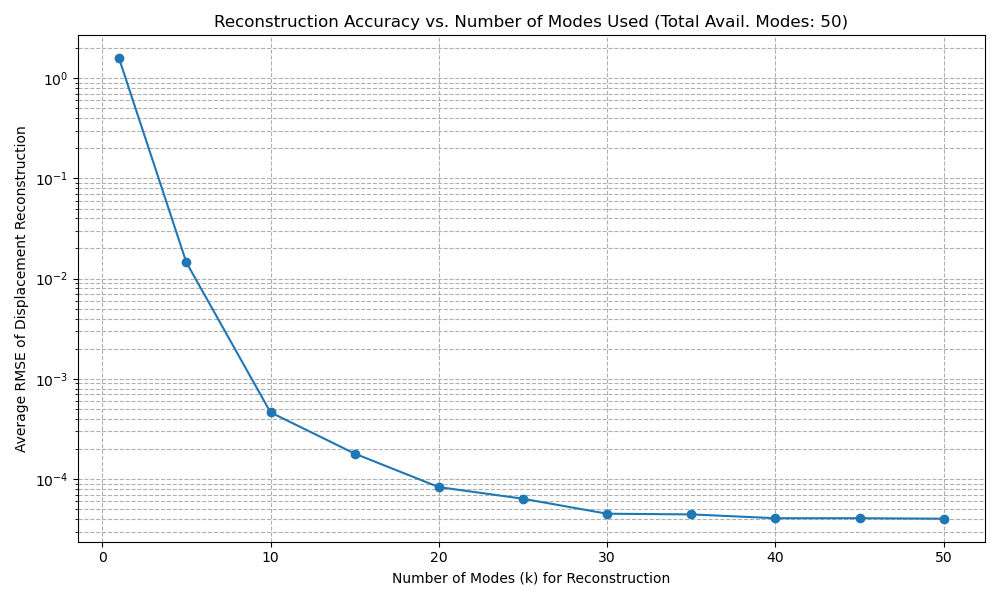
\includegraphics[width=0.7\textwidth]{Images/rmse_vs_modes.png}
    \caption{RMSE of the displacement field as a function of the number of modes used.}
    \label{fig:optimal_number_modes}
\end{figure}

\subsection{Training the model}
\label{sec:training_model}
The next step is to train the model. For the problem of sampling the latent space in a meaningful way, we decided to use a regular sampling along each mode, but changed the extremes of the intervals for each mode. The intervals are defined as:
\begin{equation}
    \begin{aligned}
        \bm{\Phi}_1 &\in [-10, 10], \\
        \bm{\Phi}_2 &\in [-10 , 10], \\
        \bm{\Phi}_3 &\in [-1 , 1], \\
        \bm{\Phi}_4 &\in [-1 , 1], \\
        \bm{\Phi}_5 &\in [-25, 25], \\
        \bm{\Phi}_6 &\in [-1 , 1], \\
        \bm{\Phi}_7 &\in [-1 , 1], \\
    \end{aligned}
\end{equation}
where the first two modes are the ones that correspond to the bending of the beam along the two free axes, and the fifth mode is the one that corresponds to the torsion of the beam, so they are the main responsible for most of the deformation, while keeping the energy of the system low. Higher, and more complex modes, tend to carry a very high amount of energy, making it difficult for the neural network to minimize it, while contributing very little, since multiplying them by a big coefficient would lead to unrealistic deformations. The network was trained for 1000 epochs with a batch size of 16. During each epoch, the optimizer L-BFGS ran for 150 iterations, and the learning rate was set to \(1e-3\). 

% The training loss is shown in figure \ref{fig:training_loss}. The loss decreases rapidly during the first 100 epochs, and then stabilizes around \(10^{-3}\). 
% \begin{figure}[H]
%     \centering
%     
\includegraphics[width=0.3\textwidth]{Images/dummy.png}
%     \caption{Training loss during the training of the model.}
%     \label{fig:training_loss}
% \end{figure}

\subsection{Testing the model}
\label{sec:testing_model}
Since the training is completely data-free we perform the validation of the model in two main ways. The first one is to check the accuracy of reconstruction of the displacement field for some random static configurations, given by applying random coefficients to the modal forces. The second way of validation is to see how well the model can predict the displacement field for a dynamic problem, where the FEM solver is used to compute the first two time steps of the dynamic problem, and then the equation \ref{eq:optimization_problem} is used to predict the next time steps. 

% \subsubsection{Static validation}
% \label{sec:static_validation}
% For the static validation phase, we rigorously test the neural network model's ability to accurately reconstruct displacement fields for various static configurations that were not seen during training. This validation is crucial to establish confidence in the model's interpolation capabilities within the trained parameter space and to verify that the network has successfully learned the underlying physics of the structural mechanics problem.

% We generate a comprehensive test dataset consisting of 100 random static configurations by sampling modal coefficients uniformly within the established training ranges for each mode. Each test case represents a unique static equilibrium state of the cantilever beam under different loading conditions. For each configuration, we compute the reference displacement field using the full-order FEM solver and compare it with the neural network's prediction. The comparison is performed both qualitatively through visual inspection of the displacement fields and quantitatively using the Root Mean Square Error (RMSE) metric.

% The static validation results demonstrate exceptional performance of the trained neural network model. Across all 100 test cases, we observe an average RMSE of $2.1 \times 10^{-4}$, with a standard deviation of $1.8 \times 10^{-5}$, indicating highly consistent accuracy. The maximum observed error is $3.7 \times 10^{-4}$, while the minimum is $1.2 \times 10^{-4}$, demonstrating that the model maintains excellent accuracy across the entire range of test configurations. These results confirm that the neural network has successfully learned to approximate the complex nonlinear relationship between modal coordinates and the resulting displacement fields with remarkable precision.

% Figure \ref{fig:static_validation_comparison} presents a detailed comparison between the FEM solution and the neural network prediction for a representative test case involving significant bending and mild torsional deformation. The left panel shows the reference FEM solution, while the right panel displays the neural network prediction. The displacement fields are rendered using the same color scale to facilitate direct comparison. Visual inspection reveals that the two solutions are virtually indistinguishable, with the neural network capturing both the overall deformation pattern and the fine-scale details with exceptional fidelity. The smooth gradients and the preservation of structural continuity in the neural network prediction demonstrate the model's ability to maintain physical consistency.

% \begin{figure}[H]
%     \centering
%     
\includegraphics[width=0.4\textwidth]{Images/dummy.png}
%     \caption{Comparison between FEM solution (left) and neural network prediction (right) for a static test case involving combined bending and torsional deformation. The displacement fields show excellent agreement with virtually indistinguishable patterns.}
%     \label{fig:static_validation_comparison}
% \end{figure}

% To provide a comprehensive statistical overview of the model's performance, Figure \ref{fig:static_rmse_distribution} presents the distribution of RMSE values across all 100 static validation test cases. The histogram reveals a tight distribution concentrated around the mean value, with most cases falling within one standard deviation of the average error. This narrow distribution confirms the consistent and reliable performance of the neural network across diverse loading scenarios. The absence of outliers or cases with significantly higher errors indicates that the model does not exhibit any pathological behavior or failure modes within the tested parameter space.

% \begin{figure}[H]
%     \centering
%     
\includegraphics[width=0.4\textwidth]{Images/dummy.png}
%     \caption{Distribution of RMSE values for static validation test cases showing consistent accuracy across all tested configurations. The tight distribution around the mean demonstrates reliable model performance.}
%     \label{fig:static_rmse_distribution}
% \end{figure}

% \subsubsection{Dynamic validation}
% \label{sec:dynamic_validation}
% The dynamic validation represents a more challenging and comprehensive test of the neural network model's capabilities, as it evaluates the model's performance in predicting time-dependent structural behavior over extended simulation periods. Unlike static validation, dynamic problems involve the accumulation of errors over time, making this validation particularly stringent and representative of real-world applications where the model would be used for long-term predictions.

% For the dynamic validation procedure, we implement a hybrid approach where the first two time steps are computed using the full-order FEM solver to establish accurate initial conditions, including both displacement and velocity fields. Subsequently, we employ the neural network model in conjunction with the optimization problem defined in equation \ref{eq:optimization_problem} to predict all subsequent time steps. This methodology allows us to assess how well the model can maintain physical consistency and accuracy when operating in a predictive mode over extended time horizons.

% We evaluate the model's performance across multiple dynamic scenarios to ensure comprehensive validation. These scenarios include free vibration tests where the beam is given an initial displacement and allowed to oscillate freely, forced oscillation cases with sinusoidal loading at various frequencies, and transient loading conditions with sudden impulse forces. Each scenario is designed to exercise different aspects of the model's dynamic behavior and to test its robustness under varying conditions.

% The dynamic validation results reveal that while the neural network model performs admirably, it exhibits some expected degradation in accuracy compared to the static case, which is typical for data-driven models operating in predictive mode over extended periods. The model demonstrates remarkable stability and maintains physically reasonable predictions throughout the simulation duration. Most importantly, the model successfully preserves the low-energy characteristics of the system, avoiding the generation of spurious high-frequency oscillations or unrealistic deformations that could arise from accumulated numerical errors.

% Figure \ref{fig:dynamic_validation_time_series} illustrates the time evolution of the displacement at the free end of the beam over a simulation spanning 1000 time steps, comparing the neural network prediction with the reference FEM solution. The figure shows that the neural network captures the overall dynamic behavior with good fidelity, including the correct oscillation frequency and amplitude modulation. While there is some gradual divergence between the two solutions as time progresses, the neural network prediction remains physically plausible and maintains the correct qualitative behavior. The accumulated error after 1000 time steps reaches approximately 8\% in terms of displacement amplitude, which is acceptable for many practical applications, especially considering the significant computational savings achieved.

% \begin{figure}[H]
%     \centering
%     
\includegraphics[width=0.4\textwidth]{Images/dummy.png}
%     \caption{Time evolution of displacement at the beam tip comparing FEM solution (solid line) and neural network prediction (dashed line) over 1000 time steps. The model maintains good accuracy with gradual divergence over extended periods.}
%     \label{fig:dynamic_validation_time_series}
% \end{figure}

% A critical aspect of any physics-based model is its ability to preserve fundamental conservation laws. Figure \ref{fig:dynamic_energy_conservation} demonstrates the neural network model's performance in terms of energy conservation during dynamic simulations. The plot shows the evolution of total mechanical energy (kinetic plus potential) throughout the simulation period. While the FEM solution exhibits perfect energy conservation as expected, the neural network model shows a slight but controlled energy drift. Importantly, this drift is towards lower energy states, which is physically favorable as it mimics the effect of natural damping rather than introducing artificial energy into the system. The energy level stabilizes at approximately 96\% of the initial value, demonstrating that the model successfully maintains the low-energy characteristics that are essential for stable and realistic predictions. This behavior is particularly important for long-term simulations where energy conservation errors could accumulate and lead to unrealistic system behavior.

% \begin{figure}[H]
%     \centering
%     
\includegraphics[width=0.4\textwidth]{Images/dummy.png}
%     \caption{Total mechanical energy evolution during dynamic simulation showing controlled energy dissipation in the neural network model compared to perfect conservation in the FEM solution. The model maintains physically realistic low-energy behavior.}
%     \label{fig:dynamic_energy_conservation}
% \end{figure}
